\chapter{Fallstudie Dynamische Learning-NFTs}

In diesem Kapitel wird das Konzept eines Learning \ac{NFT}s im Rahmen einer Fallstudie analysiert und erläutert.
Basis der Analyse bietet hierbei der von Peter C. Evans entwickelte MyLearning\ac{NFT} \parencite[vgl.][]{MyLearningNFT.2022}.
Nach Erläuterung der Funktionsweise sollen verbesserte Einflussmöglichkeiten auf einen nachhaltigen Lernprozess aufgezeigt werden und wie diese Daten Institutionen helfen können.
Dann wird auf die Besonderheit eines dynamischen \ac{NFT} eingegangen und welche Vorteile die Blockchain bezüglich Fälschungssicherheit, Transparenz und Plattformunabhängigkeit bieten kann.
Abschließend wird zudem der Trend um \ac{NFT}s und Blockchain näher beleuchtet. 

\section{Funktionsweise}

Der dynamische MyLearning\ac{NFT} ändert seinen Status, je nachdem wie der Teilnehmer nach einer abgeschlossenen Schulung oder Fortbildung weiterlernt.
Dabei gibt es zwei Hauptaspekte:
Zum einen gibt es Lernaktivitäten die bezeichnen wie der Teilnehmer lernt,
beispielsweise durch Lesen eines Artikels oder das Hören eines Podcasts.
Zum anderen die Wissensbereiche, also die Themen, die ein Teilnehmer im Anschluss an ein Lernevent weiter vertiefen und lernen soll.
Diese Daten werden bereits vor Beginn des Kurses durch den Veranstalter vorbereitet
und können nach dem Event über den Account eines jeden Nutzers auf der Webseite eingetragen werden und müssen dann vom Veranstalter validiert werden.
Der Nutzer bekommt für die Lernaktivität dann eine bestimmte Anzahl von Punkten gutgeschrieben, welche wiederum den Score verändert und eine Einteilung in 5 Stufen ermöglicht, siehe Abbildung \ref{stufen} \parencite[vgl.][]{MyLearningNFT.2022}.

\begin{figure}[ht]
    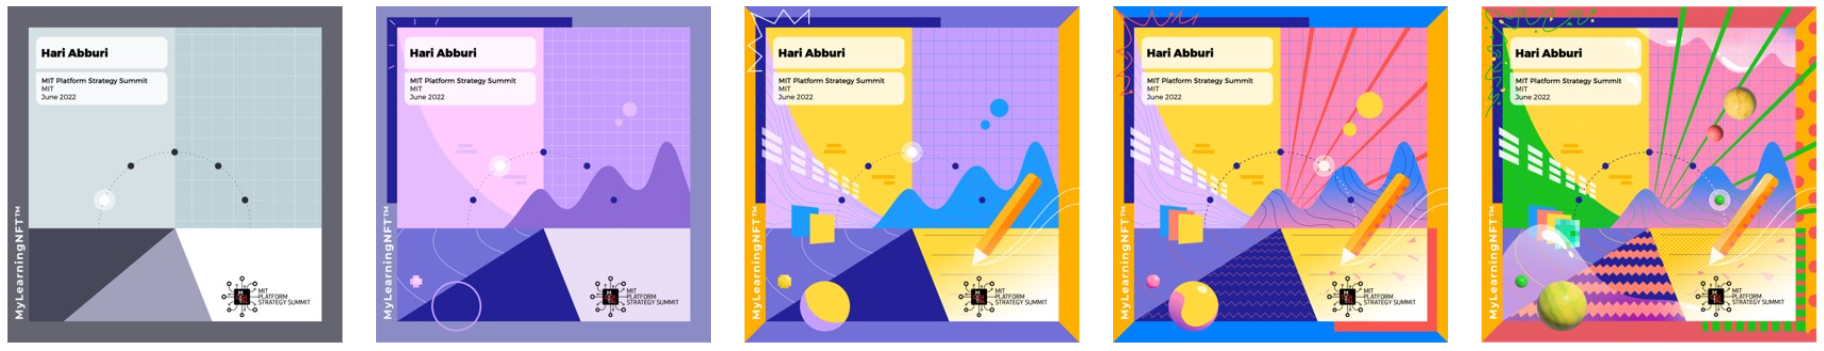
\includegraphics[width=15.8cm]{Bilder/Stufen.PNG}
    \centering
    \captionabove[Stufen 1-5 des MyLearningNFT]{Stufen 1-5 des MyLearning\ac{NFT} \parencite[vgl.][]{MyLearningNFT.2022}}
    \label{stufen}
\end{figure}

Direkt nach dem Event startet der Teilnehmer mit 50 Punkten, was der mittleren Stufe entspricht.
Lernt ein Teilnehmer innerhalb von 90 Tagen nach einem Lernevent weiter und sammelt Punkte, so behält der \ac{NFT} seinen Status oder erhöht sich.
Bleibt der Teilnehmer nach dem Event nicht an dem Thema dran und macht keine Auffrischungen, weiterführende Lerneinheiten o.ä. wird davon ausgegangen,
dass der Teilnehmer, wie von Ebbinghaus beschrieben, Stück für Stück mehr des gelernten wieder vergisst.
Beim \ac{NFT} sinkt dann über die Zeit das Punktekonto und der \ac{NFT} ändert den Status negativ \parencite[vgl.][]{MyLearningNFT.2022}.

\section{Nachhaltiges Lernen}

Um den Status des \ac{NFT} auf einer hohen Stufe zu halten, muss sich der Teilnehmer immer wieder aktiv mit dem Thema Auseinandersetzen.
Diese Lernmethode der Wiederholung sorgt dafür, dass erlerntes Wissen nachhaltiger gespeichert und zu einem späteren Zeitpunkt wieder abgerufen werden kann \parencite[vgl.][221-223]{Sattler.2009}
und wirkt der Vergessenskurve nach Ebbinghaus damit entgegen.
Der Teilnehmer kann einen deutlich größeren Anteil der Inhalte über einen längeren Zeitraum behalten und erworbenes Wissen nachhaltig eingesetzt werden.
Der Wert der Lernaktivität ist damit über einen längeren Zeitraum gesehen um einiges höher (siehe Abbildung \ref{forg}).

\begin{figure}[h]
    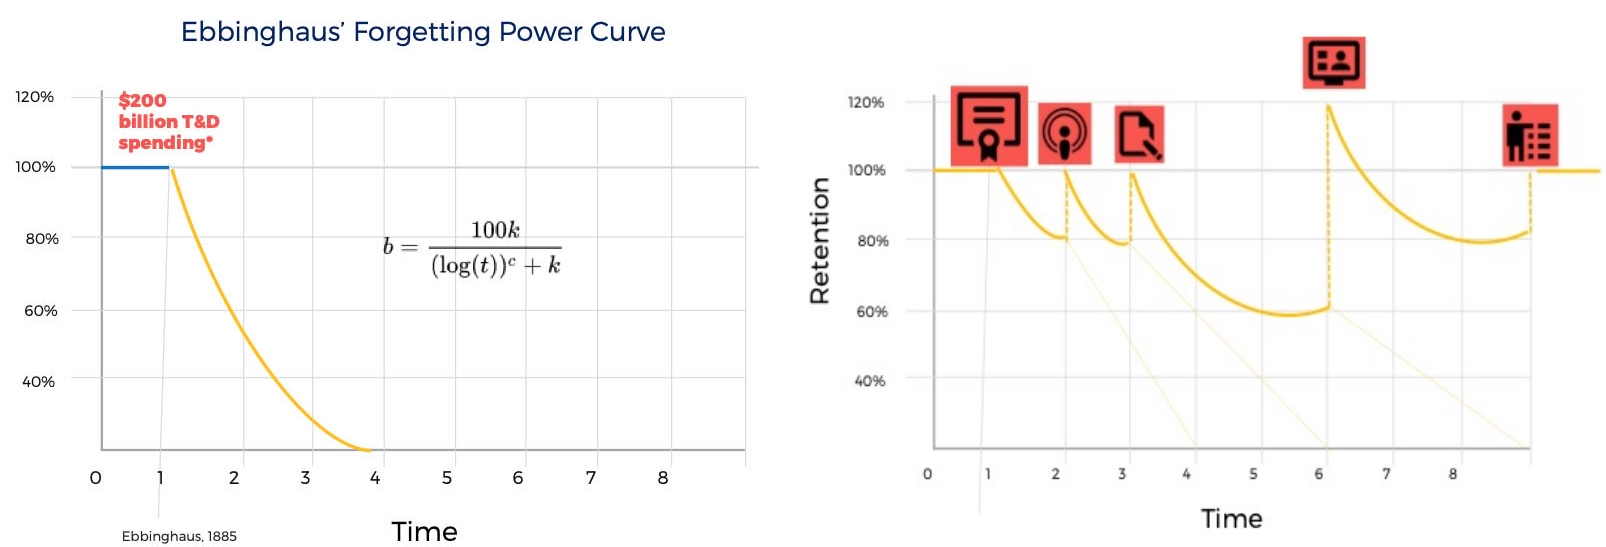
\includegraphics[width=15.8cm]{Bilder/EbinghausForgeting.png}
    \centering
    \captionabove[Vergessenskurve mit Verwendung des MyLearningNFT]{Vergessenskurve normal (links) und mit beispielhafter Verwendung des MyLearning\ac{NFT} (rechts) \parencite[vgl.][]{MyLearningNFT.2022}}
    \label{forg}
\end{figure}

Verknüpfungen von Schulungen und Fortbildungen mit dem MyLearning\ac{NFT} können einen großen Einfluss auf nachhaltiges Verinnerlichen der Inhalte haben.
Eine, im Vergleich zum Lernevent, kleine zusätzliche Investitionen von 1\% bis 3\% in einen Learning \ac{NFT} kann die Effektivität des Events damit erheblich steigern
und ist auch aus ökonomischer Sicht sehr sinnvoll \parencite[vgl.][]{MyLearningNFT.2022}.

\section{Datenerhebung zum Lernverhalten}

Der Mangel an Daten zum Lernverhalten ist ein weiteres Problem das gelöst werden kann.
Institutionen und Unternehmen können kaum Daten über das Lernverhalten der Teilnehmer nach einem Kurs oder Seminar sammeln
oder wie sie sich über den Kurs hinaus weiter mit dem Thema beschäftigen und weiter lernen.
Das Analysetool des MyLearning\ac{NFT} kann Unternehmen dabei helfen zu verstehen wie die Teilnehmer nach dem Event lernen und in welchen Themengebieten.
Mit diesen Informationen kann Veranstaltern und Unternehmen geholfen werden zukünftige Schulungen und Seminare besser anzupassen und ausrichten zu können.
Die Vorteile liegen klar auf der Hand:
Das Event kann für den Teilnehmer effektiver gestaltet werden.
Zum anderen kann das Ereignis der Investition in Lerneinheiten und Entwicklungsprogramme erheblich gesteigert werden \parencite[vgl.][]{MyLearningNFT.2022}.

\section{Dynamische NFTs}

Im Grundlagenkapitel wurde bereits erklärt wie basierend auf der Blockchain in Verbindung mit Smart Contracts ein \ac{NFT} funktioniert.
Ein dynamischer \ac{NFT} stellt wiederum eine kleine Besonderheit dar.
Denn \dq normale\dq{} \ac{NFT}s, wie zum Beispiel das Besitzzertifikat für ein digitales Kunstwerk, sind statisch und können nicht verändert werden.
Durch die Einführung von Layer-2-Skalierung ist es aber möglich geworden spezifische Tokens zu erstellen,
die mit der Blockchain verknüpft sind und durch bestimmte Events geändert werden können.
Realisiert wird das durch die Einführung von Side-Chains, welche mit dem Hauptzweig verbunden sind.
Diese Child-Blockchains oder auch Plasma-Blockchains speichern gelegentlich einen Fingerabdruck der Plasma-Chain auf die Root-Blockchain \parencite[vgl.][]{BitcoinSuisse.2020}.
Im Fall vom MyLearning\ac{NFT} wäre das die Ethereum-Blockchain \parencite[vgl.][]{MyLearningNFT.2022}.
Die Reduzierung der Daten für die Root-Chain verkürzt Transaktionen und spart damit Kosten.
Auch kann das Konsensverfahren auf der Plasma-Chain angepasst und spezifisch an die Anforderungen des dynamischen \ac{NFT} angepasst werden \parencite[vgl.][]{BitcoinSuisse.2020}.

Den \ac{NFT} in seinem Wert dynamisch anpassen zu können ermöglicht das \dq Wissenslevel\dq{} des Teilnehmers aktuell darzustellen.
Herkömmliche gamifizierte Lernplattformen wie die aktuelle SAP Experience Garage Technology Plattform arbeiten mit dem Prinzip eines sich nur positiv ändernden Score der immer weiter steigt.
%Ein solch steigender Score motiviert den Mitarbeiter zwar in erster Hinsicht mehr, weil er einen ständigen Anstieg seiner Punkte sieht.
Aussagekraft über sein \dq Wissenslevel\dq{} hat der Wert jedoch kaum.

Angenommen ein Benutzer hat vor vier Jahren einen Python-Workshop mitgemacht, fünf Lerneinheiten abgeschlossen und an zwei Projekten mitgearbeitet.
Danach hat er bis heute, über einen Zeitraum von drei Jahren, keine Berührung mehr mit der Programmiersprache gehabt.
Den Score, den er dafür vor drei Jahren bekam, hat heute immer noch denselben Punkte-Wert. 
Aktualität hat dieser jedoch Wert nicht mehr, ebenso wenig eine sinnvolle Vergleichbarkeit oder sichtbare Qualifizierungsmöglichkeit.
Denn die Programmiersprache hat sich weiter entwickelt und der Teilnehmer hat viel des gelernten vergessen und ist nicht mehr abrufbar, siehe Abbildung \ref{forg}.
Ein Score, der das aktuelle \dq Wissenslevel\dq{} des Teilnehmers widerspiegelt, hätte für Nutzer daher eine deutlich höhere Relevanz und könnte für bessere Vergleichbarkeit der Teilnehmer sorgen,
als auch eine Möglichkeit bieten, Teilnehmer ein aktuelles Skill-Level zu bescheinigen beziehungsweise zertifizieren zu können.

\section{Fälschungssicherheit und Transparenz} \label{fundt}

Einen zusätzlichen Gewinn für den Benutzer stellt die Fälschungssicherheit und Transparenz dar.
Für Fälschungssicherheit sorgt die ständige Protokollierung der Transaktionen in der Blockchain, durch welche es nicht mehr möglich ist eine Transaktion nachträglich zu manipulieren.
Transparenz entsteht durch die Öffentlichkeit der Blockchain, welche die Möglichkeit bietet, alle Transaktionen zurückverfolgen und prüfen zu können \parencite[vgl.][13]{WILKENS.2019}.

Der Nutzer eines MyLearning\ac{NFT} kann also sicher sein das seine Daten manipulationssicher gespeichert sind und geben ihm ein hohes Sicherheitsgefühl und Vertrauen in den Learning-\ac{NFT}.

\section{Plattformunabhängigkeit}

Dass der Learning-\ac{NFT} in einer öffentlichen Blockchain gesichert ist, macht ihn das zudem Plattformunabhängig.
Zum einen hat das den Vorteil, dass wenn die Ursprünglich genutzte Plattform abgeschaltet wird,
der Learning-\ac{NFT} weiter existieren und dank Smart Contracts auch weiterhin mit neuen Daten gefüttert werden kann.
Zum anderen kann der \ac{NFT} auch von anderen Plattformen durch die Smart Contracts genutzt werden.

Diese Plattformunabhängigkeit zusammen mit den bereits erwähnten Vorteilen bezüglich Fälschungssicherheit und Transparenz
eines Learning-\ac{NFT} schafft ein großes Potenzial dem Learning-\ac{NFT} eine weitreichendere Wirkung zu verleihen
und ein aussagekräftiges \dq Wissenslevel\dq{} des Teilnehmers in verschiedenen Kategorien bereitzustellen.
Der Learning-\ac{NFT} könnte hier eine neue sichere und immer aktuelle Möglichkeit eines Lernzertifikats darstellen.

\section{Blockchain und NFTs: Hype oder Zukunft}

Nicht zu unterschätzen ist in Bezug auf \ac{DLT}, Blockchain und \ac{NFT}s auch der Einfluss des Hypes um die Technologien.
Kaum ein Markt ist in den letzten Jahren so gewachsen wie diese.
Allein \ac{NFT}s sind mit einem Handelsvolumen von 2 Milliarden USD im ersten Quartal 2021 auf 16,5 Milliarden USD ein Jahr später gestiegen.
Auch die Anzahl an Krypto-Wallets ist in diesem Zeitraum explodiert und hat sich verzehnfacht \parencite[vgl.][]{NonFungible.2022}.
Der Marktbericht von Verified Market Research geht sogar davon aus das die Branche bis 2030 durchschnittlich um 33,7\% jährlich wächst und auf ein Volumen von 231 Milliarden USD ansteigt \parencite[vgl.][]{VerifiedMarketResearch.2022}.
Ähnliche Prognosen gibt auch SkyQuest ab \parencite[vgl.][]{Skyquest.2022}.

Auch in der Öffentlichkeit sind Blockchain und \ac{NFT}s immer mehr ein Begriff \parencite[vgl.][]{PSW.2022}.
Blockchain hat ein gutes Image und wird als sicherer Ort für revisionssichere Speicherung gesehen.
Bei \ac{NFT}s gehen die Meinungen etwas weiter auseinander.
Technisch weniger versierte Menschen sind verwirrt, warum man digitale Bilder und Accessoires als einen \ac{NFT} kauft und was man überhaupt damit machen sollte.
Menschen, die sich mit dem Thema beschäftigt haben oder sich im Bereich neuer Technologien bewegen, können damit schon mehr anfangen und sehen große Potenziale und welchen Nutzen NFTs mit sich bringen \parencite[vgl.][]{vparthier.23.04.2022}.

Ein Lernzertifikat als einen \ac{NFT} ausgestellt zu bekommen ruft dabei für den Benutzer ein innovatives und sicheres Gefühl hervor und strahlt einen hohen Wert aus.
Diese positive Wahrnehmung wirkt sich wiederum vorteilhaft auf die Lernaktivität aus und hilft bei der Anerkennung und Verbreitung des Learning-\ac{NFT}. 

